\documentclass{beamer}

\usepackage{moy-slides}
\usepackage{tikz}
\usepackage{comment}
\usepackage{listings}
\usepackage{array}

\title[Pagai]{The Pagai tool}

\subtitle{Path Analysis for the Generation of Arithmetic Invariants} % (optional)

\author[J. Henry, D. Monniaux, M. Moy]{\underline{Julien Henry}, David Monniaux, Matthieu
Moy}
% - Use the \inst{?} command only if the authors have different
%   affiliation.

\newcommand{\important}[1]{\color{trefle}{#1}}

\institute[Verimag]{

\includegraphics[height=1.1cm]{../report/images/logoverimag}}

\tikzstyle{arrow}=[->,line width=.05cm,draw=red!90!blue!60!black]

\usetikzlibrary{fit}					% fitting shapes to coordinates
\usetikzlibrary{snakes,arrows,shapes,backgrounds,shadows,automata,patterns}
%\date{}
\usepgflibrary{snakes}

\tikzstyle{state}=[circle,fill=black!25,minimum size=13pt,inner sep=0pt]
\tikzstyle{bb}=[rectangle,fill=black!15,minimum size=13pt,inner sep=0pt]
\tikzstyle{transition}=[->,rectangle,thick,draw=black!75,
  			  fill=black!20,minimum size=4mm]
\tikzstyle{transition2}=[->,rectangle,thick,draw=blue!75,
  			  fill=blue,minimum size=4mm,blue]
\tikzstyle{PRstate}=[circle,fill=red!90,minimum size=13pt,inner sep=0pt]
\tikzstyle{polyhedra}=[blue!25,opacity=0.5,pattern=north west lines,pattern
color=blue]
\tikzstyle{line}=[black,thick]
\tikzstyle{NewPath}=[rectangle,thick,draw=black!75,
  			  fill=black!20,minimum size=4mm,dash pattern=on 3pt off 3pt]
\tikzstyle{TakenPath}=[rectangle,thick,draw=blue!75,
  			  fill=blue,minimum size=4mm,blue]


\begin{document}

\begin{frame}
  \titlepage
\end{frame}

\begin{frame}
	\frametitle{Pagai}

	\begin{center}
	Computes numerical invariants from an LLVM bitcode file
	\end{center}

	\vspace{1cm}

	LLVM bitcode is generated by clang or llvm-gcc :
	\begin{itemize}
		\item clang supports C and C++
		\item llvm-gcc supports C, C++, Fortran and Ada
	\end{itemize}
\end{frame}

\begin{frame}
	\frametitle{LLVM IR}
\begin{columns}
	\lstinputlisting{halbwachs-simple.c}
\begin{column}{1cm}
\end{column}
\begin{column}{10cm}
	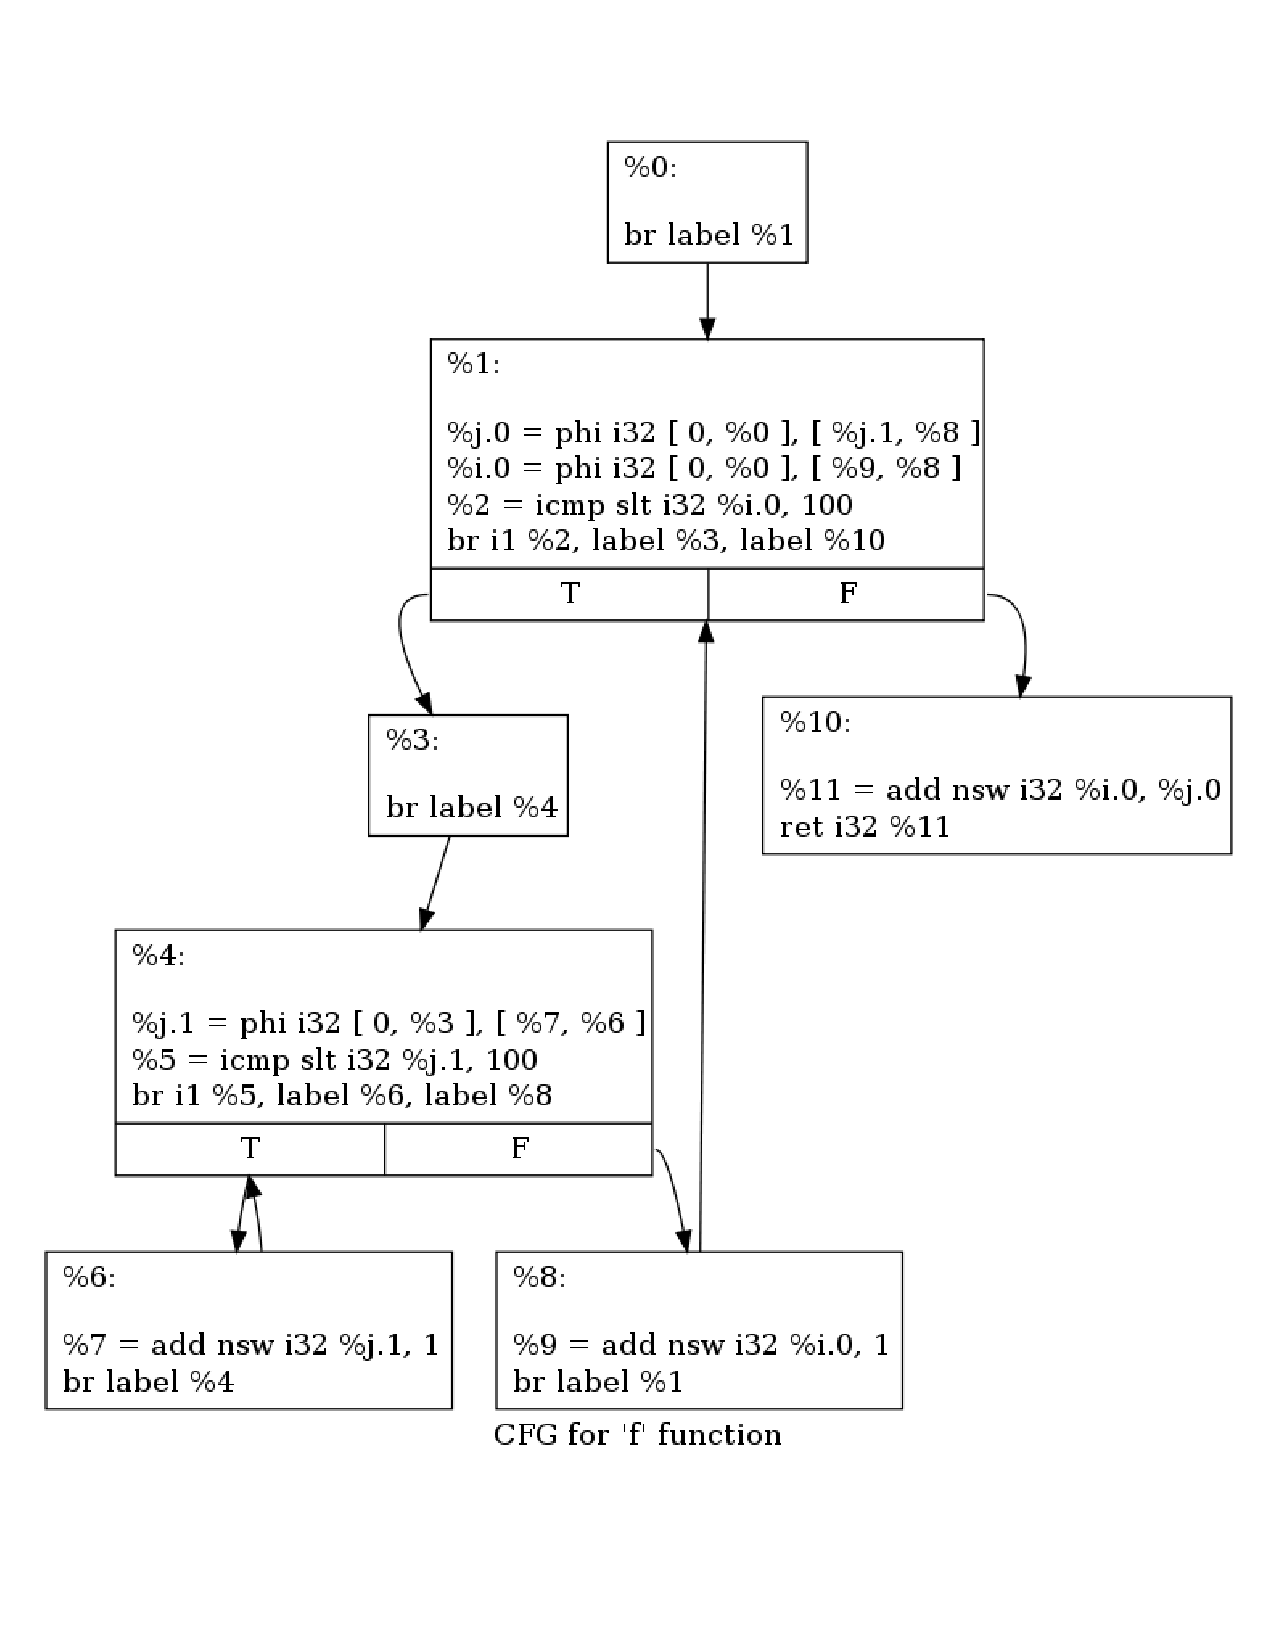
\includegraphics[width=7cm]{f.pdf}
\end{column}
\end{columns}

\end{frame}

\begin{frame}
	\frametitle{Principle}

	Computes an invariant at the head of each BasicBlock

	\vspace{1cm}

	\begin{itemize}
		\item The invariant is only on live values.
		\item Computes the image of an abstract value by a path/transition in
			one ``big'' step.
	\end{itemize}
\end{frame}

\begin{frame}[containsverbatim]
	\frametitle{Example}
For each loop header, Pagai returns an invariant in the following form:
	\begin{verbatim}
RESULT FOR BASICBLOCK: -------------------
; <label>:1 
  %j.0 = phi i32 [ 0, %0 ], [ %j.1, %8 ]
  %i.0 = phi i32 [ 0, %0 ], [ %9, %8 ]
  %2 = icmp slt i32 %i.0, 100
  br i1 %2, label %3, label %10
-----
polyhedron of dim (2,0)
array of constraints of size 3
 0: -i.0 + j.0 >= 0
 1: -j.0 + 100 >= 0
 2: 100i.0 - j.0 >= 0
\end{verbatim}
\end{frame}

\begin{frame}[containsverbatim]
	\frametitle{Assert}
Pagai can check that an assert is always true / may be wrong.
\begin{columns}
	\lstinputlisting{gopan_assert.c}
\begin{column}{1cm}
\end{column}
\begin{column}{10cm}
\begin{verbatim}
RESULT FOR BASICBLOCK: ------
; <label>:15                                      
  call void @assert_fail(...) 
  unreachable
-----
empty polyhedron of dim (0,0)
ASSERT OK
\end{verbatim}
\end{column}
\end{columns}
\end{frame}

\begin{frame}
	\frametitle{SMT solvers}
	Pagai uses SMT solvers for Path-focusing techniques

	\begin{itemize}
		\item Yices
		\item Microsoft Z3
	\end{itemize}

	In practice, Z3 is better.
\end{frame}

\begin{frame}
	\frametitle{Apron}
B. Jeannet and A. Mine. CAV'2009. 

\vspace{1cm}

Apron is a numerical abstract domain library.

\begin{itemize}
	\item BOX intervals library
	\item OCT octagon library
	\item NEWPOLKA Convex Polyhedra and Linear Equalities library 
\end{itemize}
Also provides an interface to the Parma Polyhedra Library
\end{frame}

\begin{frame}
	\frametitle{Techniques implemented}

	\begin{itemize}
		\item Classic Abstract interpretation
		\item Guided static analysis (Gopan \& Reps SAS'07)
		\item Path Focusing (Monniaux \& Gonnord SAS'11)
		\item Combined technique
		\item Combined technique with disjunctive invariants
	\end{itemize}

\end{frame}

\begin{frame}
	\frametitle{Limitations}

	\begin{itemize}
		\item no memory model
			\begin{itemize}
				\item LOAD $x \Rightarrow x \in (-\infty,+\infty)$   
				\item STORE $x$ does nothing 
			\end{itemize}
		\item intraprocedural
			\begin{itemize}
				\item a function call has the same effect than a LOAD
			\end{itemize}
	\end{itemize}

	\vspace{1cm}
	
	Remark : We use an LLVM pass (mem2reg) that 
	lifts most memory accesses to scalar variables.
\end{frame}

\begin{frame}
	\frametitle{Experiments}

	Various experiments have been done :

	\begin{itemize}
		\item benchmarks for WCET analysis or termination
		\item various GNU programs 
			\begin{itemize}
				\item grep, gnuchess, gnugo, gzip, etc.
			\end{itemize}
	\end{itemize}
\end{frame}

\begin{frame}
	\frametitle{Scalability}

\begin{table}[!h]
	\centering
\begin{tabular}{|l|r|r||r|r|r|r|r|} \hline
	 	 & & &
        \multicolumn{5}{|c|}{Time (in seconds)} 
		\\ \cline{4-8}
		Name & kLOC & $ |loops| $ & S & G & PF & C & DIS \\ \hline
		a2ps-4.14 & 46 & 11 & 45 & 127 & 280 \\
gawk-4.0.0 & 54 & 7 & 14 & 34 & 60 \\
gnuchess-6.0.0 & 164 & 21 & 121 & 411 & 1217 \\
gnugo-3.8 & 222 & 36 & 129 & 398 & 942 \\
grep-2.9 & 40 & 14 & 18 & 50 & 177 \\
gzip-1.4 & 60 & 12 & 40 & 123 & 309 \\
lapack-3.3.1 & 594 & 202 & 2769 & 6897 & 11136 \\
make-3.82 & 22 & 8 & 33 & 90 & 173 \\
sed-4.2 & 42 & 9 & 37 & 154 & 371 \\
tar-1.26 & 275 & 40 & 114 & 316 & 722 \\

	\hline
\end{tabular}
\label{fig:projects}
\end{table}

\end{frame}

\begin{frame}
	\begin{center}
		Thank you.
	\end{center}
\end{frame}
\end{document}

%%% Local Variables:
%%% mode: latex
%%% TeX-master: t
%%% ispell-local-dictionary: "american"
%%% End:
